
\chapter{Hashes}
\label{hashes}

This chapter presents another built-in type called a hash. 
Hashes are one of Raku's best and most commonly used 
features; they are the building blocks of many efficient 
and elegant algorithms.


\section{A Hash is a Mapping}
\label{hash_descr}

\index{hash}
\index{type!hash}
\index{key}
\index{key-value pair}
\index{index}
\index{mapping}
A {\bf hash} is like an array, but more general.  In an 
array, the indices or subscripts have to be integers; in a hash, 
they can be (almost) anything.

A hash contains a collection of indices, which are called 
{\bf keys}, and a collection of values.  Each key is associated with a single value.  A key and a value together form a pair 
(an object of the {\tt Pair} type), or a {\bf key-value pair}. A
hash can be viewed as a collection of key-value pairs. The 
values in a hash can also be called items or elements, as with arrays.
\index{item}

In other programming languages, hashes are sometimes called 
dictionaries, hash tables, maps, or associative arrays.

In mathematical language, a hash represents a {\bf mapping}
from keys to values, so you can also say that each key
``maps to'' a value. As an example, we'll build a hash that 
maps from English to Spanish words, so the keys and the 
values are all strings.

In Raku, hash names start with the ``\verb"%"'' sigil. To create 
a new hash, you just declare it this way:
\index{sigil}
\index{sigil, percent}

\begin{verbatim}
> my %eng2sp;
\end{verbatim}

This creates an empty hash. To add items to the hash, 
you can use curly braces (a.k.a. curly brackets and 
sometimes simply ``curlies''):
\index{curly bracket}
\index{bracket!curly}
\index{brace}

\begin{verbatim}
> %eng2sp{'one'} = 'uno';
uno
\end{verbatim}
%
This line creates an item that maps from the key
\verb"'one'" to the value \verb"'uno'".  

If the key is a string containing a single word (i.e., 
without any space in the middle of it), there is a more 
idiomatic shortcut to create the same hash entry:
\index{idiomatic}

\begin{verbatim}
> %eng2sp<one> = 'uno';
uno
\end{verbatim}
%

If we print the hash, we see a key-value pair with a 
\verb'=>' pair constructor operator between the key 
and value:
\index{pair constructor}

\begin{verbatim}
> say %eng2sp;
one => uno
\end{verbatim}
%
This output format is also an input format.  For example,
you can create a new hash with three items:

\begin{verbatim}
> my %eng2sp = ('one' => 'uno', 'two' => 'dos', 'three' => 'tres');
one => uno, three => tres, two => dos
\end{verbatim}
%

Using the \verb'=>' pair constructor operator between keys and 
values is not required; you may use a comma as well:

\begin{verbatim}
my %eng2sp = ('one', 'uno', 'two', 'dos', 'three', 'tres');
\end{verbatim}
%

But the pair constructor has the advantage of showing more 
graphically the key-value relations. The pair constructor 
operator also makes the use of quotes non mandatory on its 
lefthand side (provided the key is a string with no space):

\begin{verbatim}
> my %eng2sp = (one => 'uno', two => 'dos', three => 'tres');
one => uno, three => tres, two => dos
\end{verbatim}
%

You might also use a more concise list syntax for the hash 
assignment and Raku will happily convert the list into a 
hash, provided the number of items in the input list is even:

\begin{verbatim}
> my %eng2sp = <one uno two dos three tres>;
one => uno, three => tres, two => dos
\end{verbatim}
%

You might be surprised by the output. The order of the 
key-value pairs is usually not the order in which you 
populated the hash. In general, the order 
of items in a hash is unpredictable.

But that's not a problem because the elements of a hash 
are never indexed with integer subscripts. Instead, you use 
the keys to look up the corresponding values:

\begin{verbatim}
> say %eng2sp<two>;
dos
\end{verbatim}
%
The key \verb"two" always maps to the value \verb"'dos'" 
so the order of the items doesn't matter.

If the key isn't in the hash, you get an undefined value:

\begin{verbatim}
> say %eng2sp<four>;
(Any)
\end{verbatim}
%
The {\tt elems} method or function works on hashes just 
as on arrays; it returns the number of key-value pairs:
\index{elems function or method}
\index{function!elems}
\index{elems function or method}
\index{method!elems}


\begin{verbatim}
> say %eng2sp.elems;
3
> say elems %eng2sp
3
\end{verbatim}
%
The {\tt :exists} adverb also works on hashes as on 
arrays; it tells you whether something appears as 
a {\em key} in the hash (appearing as a value is not 
good enough)\footnote{Evaluating the value in a Boolean 
context would also work with our example, but this would 
return something wrong when the key exists, but the value 
is not defined or otherwise evaluates to a false value 
(for example if it is equal to {\tt False}, zero, or 
an empty string).}:
\index{membership!hash}
\index{exists adverb}
\index{adverb!:exists}

\begin{verbatim}
> %eng2sp<two> :exists;
True
> %eng2sp<four> :exists;
False
\end{verbatim}
%
To see whether something appears as a value in a hash, you
can use the {\tt values} method, which returns a collection of
values, and then use a loop (or possibly a {\tt grep}) to 
look for the searched item:
\index{values function or method}
\index{method!values}
\index{grep}

\begin{verbatim}
my @vals = values %eng2sp;
for @vals -> $value {
    say "Found it!" if $value eq 'uno';           # -> Found it!
}
\end{verbatim}
%
Or more concisely:
\begin{verbatim}
say "Found it!" if grep {$_ eq 'uno'}, %eng2sp.values;
\end{verbatim}

Since {\tt grep} defaults to a smart match, this can be 
made even more concise:

\begin{verbatim}
say "Found it!" if grep 'uno', %eng2sp.values;  # -> Found it!
\end{verbatim}

When looking for values, the program has to search the 
elements of the list in order (or sequentially), as in 
Section~\ref{find}.  As the list gets longer, the search 
time gets longer in direct proportion.
\index{sequential search}
\index{search!sequential}

By contrast, when looking for keys, Raku uses a {\bf hashing} 
algorithm that has a remarkable property: it takes about 
the same amount of time no matter how many items are in 
the hash. In other words, it performs really fast, compared 
to the list size, when the 
searched list is large. This is the reason why the solution to 
the reverse pair exercise (Exercise~\ref{reverse_pair}) of the 
previous chapter using a hash was almost three times 
faster than the bisection search solution 
(see Subsection~\ref{sol_reverse_pair}).

\label{ex_employees}
As an exercise, use the sample employee data of the 
multidimensional array of Section~\ref{multidimensional_array} 
(p.~\pageref{multidimensional_array}), load it into a hash, and 
look up some salaries. Hint: you don't need a 
multidimensional structure for doing that with a hash.
Solution: \ref{sol_ex_employees}


\section{Common Operations on Hashes}

We've seen already that to populate a hash, you can just 
assign an even list to it. The four syntactical forms 
below are correct:

\begin{verbatim}
my %first_quarter = ("jan" => 1, "feb" => 2, "mar" => 3);
my %second_quarter = (apr => 4, may => 5, jun => 6);
my %third_quarter = jul => 7, aug => 8, sep => 9;
my %fourth_quarter = < oct 10 nov 11 dec 12 >;
\end{verbatim}

To add an element to a hash, just assign the hash with a key:

\begin{verbatim}
my %months = ("jan" => 1, "feb" => 2, "mar" => 3);
%months{'apr'} = 4;
say %months;         # -> apr => 4, feb => 2, jan => 1, mar => 3
\end{verbatim}

Remember that you can also do the same without having to 
quote the keys if you use the angle brackets quote-word 
operator (if the keys are strings):
\index{quote-word operator}
\index{angle bracket}

\begin{verbatim}
%months<apr> = 4;       # same as: %months{'apr'} = 4;
\end{verbatim}

or you can also use the {\tt push} function with a pair:
\index{push function}
\index{function!push}

\begin{verbatim}
> push %months, (may => 5);
apr => 4, feb => 2, jan => 1, mar => 3, may => 5
> my $new-pair = jun => 6
jun => 6
> push %months, $new-pair;
apr => 4, feb => 2, jan => 1, jun => 6, mar => 3, may => 5
\end{verbatim}
%

Using {\tt push} to add a pair to a hash is not exactly the same, 
though, as making a hash assignment: if the key already 
exists, the old value is not replaced by the new one---instead,  
the old and the new ones are placed into an array (or, 
if the old value is already an array, then the new value 
is added to the array):

\begin{verbatim}
> push %months, (jan => '01');
{apr => 4, feb => 2, jan => [1 01], jun => 6, mar => 3, may => 5}
\end{verbatim}

To check whether a value is defined for a given key, 
use {\tt defined}:
\index{defined}

\begin{verbatim}
> say True if defined %months<apr>;
True
\end{verbatim}
%

To obtain the number of items in a hash, use the {\tt elems}
method:
\index{elems function or method}

\begin{verbatim}
say %months.elems;                # -> 6
\end{verbatim}

To remove a hash item, use the {\tt :delete} adverb:
\index{delete adverb}
\index{adverb!:delete}

\begin{verbatim}
> push %months, (jud => 7);      # Oops, a typo!
apr => 4, feb => 2, jan => 1, jud => 7, jun => 6, mar => 3, may => 5
> %months{'jud'}:delete;         # typo now removed
7
> say %months
apr => 4, feb => 2, jan => 1, jun => 6, mar => 3, may => 5
\end{verbatim}

Note that the {\tt :delete} adverb also returns the value that 
is being removed.

To iterate over a hash, use:
\index{kv function or method}
\index{keys function or method}
\index{values function or method}
\index{pairs function or method}

\begin{itemize}
\item {\tt kv} to retrieve the interleaved keys and values;
\item {\tt keys} to retrieve the keys;
\item {\tt values} to retrieve the values;
\item {\tt pairs} to retrieve the key-value pairs;
\end{itemize}

For example:

\begin{verbatim}
> for %months.kv -> $key, $val { say "$key => $val" }
jan => 1
apr => 4
mar => 3
jun => 6
may => 5
feb => 2
> say keys %months;
(jan apr mar jun may feb)
> say values %months;
(1 4 3 6 5 2)
> say %months.pairs;
(jan => 1 apr => 4 mar => 3 jun => 6 may => 5 feb => 2)
\end{verbatim}
%

\section{Hash as a Collection of Counters}
\label{histogram}
\index{counter}

Suppose you are given a string and you want to count how many
times each letter appears.  There are several ways you could do it:

\begin{itemize}

\item You could create 26 variables, one for each letter of the
alphabet.  Then you could traverse the string and, for each
character, increment the corresponding counter, probably using
an ugly and huge 26-part chained conditional.

\item You could create an array with 26 elements.  Then you could
convert each character to a number (using the built-in function
{\tt ord}), use the number as an index into the array, and 
increment the appropriate counter.

\item You could create a hash with characters as keys
and counters as the corresponding values.  The first time you
see a character, you would add an item to the hash.  After
that, you would increment the value of an existing item.

\end{itemize}

Each of these options performs the same computation, but each
of them implements that computation in a different way.
\index{implementation}

An {\bf implementation} is a way of performing a computation;
some implementations are better than others.  For example,
an advantage of the hash implementation is that we don't
have to know ahead of time which letters appear in the string
and we only have to make room for the letters that do appear.

Here is what the code might look like:

\begin{verbatim}
sub histogram (Str $string) {
    my %histo;
    for $string.comb -> $letter {
        %histo{$letter}++;
    }
    return %histo;
}
\end{verbatim}
%
The name of the function is {\tt histogram}, which is a statistical
term for a collection of counters (or frequencies).
\index{histogram}
\index{frequency}
\index{traversal}
\index{comb function and method}
\index{counter}

The first line of the
function creates an empty hash.  The {\tt for} loop traverses
the string.  Each time through the loop, if the character \verb'$letter' is
not in the hash, Raku creates a new item with key 
\verb'$letter' and defaults the values to 0 when the ``++'' 
operator is called on it, so that the first value immediately 
thereafter is 1.  If \verb'$letter'  is already in the hash,
the value is incremented.
\index{increment operator}

Here's how it works:

\begin{verbatim}
> say histogram("We all live in a yellow submarine")
W => 1, a => 3, b => 1, e => 4, i => 3, l => 5, (...) y => 1
\end{verbatim}
%
The histogram indicates that the letters \verb"'W'" and 
\verb"'b'" appear only once; \verb"'a'" and \verb"'i'" 
appear three times, \verb"'e'" appears four times, and so on.

\section{Looping and Hashes}
\index{hash!looping with}
\index{looping!with hashes}
\index{traversal}

If you use a hash in a {\tt for} statement, it traverses
the pairs of the hash:

\begin{verbatim}
> for %eng2sp -> $pair { say $pair}
two => dos
three => tres
one => uno
\end{verbatim}
%

We have named the iteration variable \verb'$pair' to point 
out more clearly that the program is iterating over key-value 
pairs (actually \verb'Pair' objects). You may use the 
{\tt key} and {\tt value} (notice the singular) methods to 
access the key and value of a \verb'Pair'. For example, to 
reverse the order in which each line is printed:

\begin{verbatim}
> for %eng2sp -> $pair { say $pair.value ~ " <= " ~ $pair.key; }
dos <= two
tres <= three
uno <= one
\end{verbatim}

Again, the keys are in no particular order.  To traverse 
the keys in sorted order, you can use the {\tt keys} 
(plural) and {\tt sort} functions or methods:
\index{keys function or method}
\index{method!keys}
\index{sort!function or method}
\index{method!sort}

\begin{verbatim}
my %histo = histogram("We all live in a yellow submarine");
for %histo.keys.sort -> $key {
    say "$key\t%histo{$key}";
}
\end{verbatim}



\section{Reverse Lookup}
\label{raise}
\index{hash!lookup}
\index{hash!reverse lookup}
\index{lookup, hash}
\index{reverse lookup, hash}

Given a hash \verb'%hash' and a key \verb'$k', it is easy to
find the corresponding value \verb'$val = %hash{$k}'.  
This operation is called a {\bf lookup} and, as already 
mentioned, this is fast even when the hash is very large.
\index{lookup}
\index{hash lookup}

But what if you have \verb'$val' and you want to find 
\verb'$k'? You have three problems: first, there might be 
more than one key that maps to the value \verb'$val'; depending 
on the application, you might be able to pick one, or you 
might have to make an array that contains all of them.  
Second, there is no simple syntax to do a {\bf reverse lookup}; 
you have to search. Third, it might be time-consuming if 
the hash is large.

Here is a function that takes a value and returns the first
key that maps to that value:	
\index{reverse lookup}

\begin{verbatim}
sub reverse-lookup (%hash, $val) { 
    for %hash -> $pair { 
        return $pair.key if $pair.value eq $val;
    }
    return;
}
\end{verbatim}
%
This subroutine is yet another example of the search pattern.
If we get to the end of the loop, that means \verb'$val'
doesn't appear in the hash as a value, so we return an 
undefined value (Nil). Here, the responsibility to react 
to that situation is left to the caller. An alternative 
might be to raise an exception, which would still have 
to be dealt with by the caller. However, since direct 
lookup with the key is not raising an exception but simply 
returning an undefined value when the key does not exist, 
it makes sense for {\tt reverse-lookup} to have the same 
behavior when the value is not found.

Here is an example of a successful reverse lookup:

\begin{verbatim}
> my %histo = histogram('parrot');
a => 1, o => 1, p => 1, r => 2, t => 1
> my $key =  reverse-lookup %histo, "2";
r
\end{verbatim}
%
And an unsuccessful one:

\begin{verbatim}
> say reverse-lookup %histo, "3";
Nil
\end{verbatim}
%

Another more concise way to do reverse lookup would be to 
use {\tt grep} to retrieve a list of values satisfying our 
condition:
\begin{verbatim}
say grep { .value == 2 }, %histo.pairs;   # -> (r => 2)
\end{verbatim}

Another option is to use an expression with the {\tt first} 
built-in function to retrieve only the first one:
\begin{verbatim}
my %histo = histogram('parrot');
say %histo.pairs.first: *.value == 1;      # ->  p => 1
\end{verbatim}

\index{whatever}
This latter example uses the ``*'' \emph{whatever} parameter 
which we haven't covered yet in this book. Let's just say that, 
here, the ``*'' stands successively for every pair of the hash, 
and the {\tt first} function returns the first pair that matches 
the condition on the value (see 
Section~\ref{whatever star parameter} for details on the 
``*'' parameter).

A reverse lookup is much slower than a forward lookup; if you
have to do it often, or if the hash gets big, the performance
of your program will suffer.
\index{reverse lookup}

\section{Testing for Existence}
\index{existence!testing for}

A quite common task is to determine whether something exists or 
if a given value has already been seen in a program. Using a 
hash is usually the best solution because finding out whether 
there is an entry for a given key is very simple and also 
very efficient: you just need to store the values that you 
want to watch as a key entry in a hash, and then check for 
its existence when needed.

In such a case, you often don't really 
care about the value and you might put basically anything. 
It is quite common in that case to use ``1'' as a value, but 
you might as well store {\tt True} or any other value you 
like.

Suppose we want to generate 10 random integers between 0 and 
49, but want to make sure that the integers are unique. We 
can use the {\tt rand} method 10 times on the desired range. But 
the likelihood to hit twice the same number is far from 
negligible (see Exercise~\ref{birthdays} on the so-called 
Birthday Paradox and its solution (Subsection~\ref{sol_birthdays}) 
for a similar situation). For example, trying this:
\index{duplicate!checking}
\index{rand function}

\begin{verbatim}
> my @list;
[]
> push @list, 50.rand.Int for 1..10;
> say @list;
[12 25 47 10 19 20 25 42 33 20]
\end{verbatim}

produced a duplicate value in the list (25) on the first try.
And the second try produced three pairs of duplicates:

\begin{verbatim}
> say @list;
[45 29 29 27 12 27 20 5 28 45]
\end{verbatim}

We can use a hash to reject any generated random integer 
that has already been seen. The following is a possible way to 
code this:
\index{rand function}

\begin{verbatim}
my @list;
my %seen;
while @list.elems < 10 {
    my $random = 50.rand.Int;
    next if %seen{$random}:exists;
    %seen{$random} = 1;
    push @list, $random;
}
say @list;
\end{verbatim}

Every valid integer generated is added to both the \verb'%seen' 
hash and the output list. But before doing 
that, the generated integer is checked against the 
\verb'%seen' hash to verify that it has not been seen yet. 
When this program is finished running, the list has 10~unique 
(pseudo-)random integers.

We have made it step by step and kept two separate data 
structures, the \verb'@list' output array and the 
\verb'%seen' hash, to make the process as clear as possible. 
If you think about it, however, \verb'@list' and \verb'%seen' 
have essentially the same content at any step through the 
loop. We don't really need to keep track of the same data in 
two places. Since having a hash is important for checking that the 
output values are unique, we can get rid of \verb'@list' 
and write a more concise and probably more idiomatic version 
of the same program:
\index{idiomatic}
\index{push function}

\begin{verbatim}
my %seen;
while %seen.elems < 10 {
	my $random = 50.rand.Int;
	push %seen, ($random => 1) unless %seen{$random}:exists;
}
say keys %seen;      # -> (39 12 46 27 14 21 4 38 25 47)
\end{verbatim}

This can be further simplified. It is not really necessary 
here to check whether the generated integer exists in the 
hash: if it does exist, the old hash element will be replaced 
by the new one, and the hash will be essentially unchanged. In 
addition, when evaluated in a scalar numeric context, a 
hash returns the number of its elements, so that the call 
to the {\tt .elems} is not necessary. This is the new version:
\index{scalar context}
\index{elems function or method}

\begin{verbatim}
my %seen;
%seen{50.rand.Int} = 1 while %seen < 10;
say keys %seen;      # -> (46 19 5 36 33 1 20 45 47 30)
\end{verbatim}

This last version is probably more concise and more idiomatic, 
but that's not meant to say that it is better. It is 
perfectly fine if you prefer the second or the first version, 
maybe because you find it clearer. Use whichever version you 
like better, or your own modified version provided it does 
the expected work. This is Raku, \emph{there 
is more than one way to do it} (TIMTOWTDI).
\index{TIMTOWTDI}

Note however that the pure hash version doesn't keep the order 
in which the numbers were generated, so (pseudo)randomness 
might not be as good.

Also note, by the way, that Raku has a {\tt pick} function or 
method to choose elements at random from a list without 
repetition.
\index{pick function or method}


\section{Hash Keys Are Unique}

It is not possible to have the same key in a hash more than once. 
Trying to map a new value to a key will replace the old 
value with the new one. Here is an example of hash creation 
with duplicates keys:
\index{duplicate}

\begin{verbatim}
> my %friends = (Tom => 5, Bill => 6, Liz => 5, Tom => 7, Jack => 3)
Bill => 6, Jack => 3, Liz => 5, Tom => 7
\end{verbatim}

Because two of our friends are named Tom, we lose the data 
associated with the first of them. This is something you should 
be careful about: hash keys are unique, so you'll lose some items  
if the data associated with your keys has duplicates. The 
next section will show some ways of dealing with this 
possible problem.

But this key uniqueness property also has very interesting upsides. 
For example, a typical way of removing duplicates from a list of 
items is to assign the list items to the keys of a hash (the 
value does not matter); at the end of the process, the list of 
keys has no duplicates:

\begin{verbatim}
> my @array = < a b c d s a z a r e s d z r a >
[a b c d s a z a r e s d z r a]
> my %unique = map { $_ => 1 }, @array;
a => 1, b => 1, c => 1, d => 1, e => 1, r => 1, s => 1, z => 1
> my @unique_array = keys %unique;
[z a e s d c b r]
\end{verbatim}

As you can see, duplicates have been removed from the output 
array. In such a simple case, the {\tt unique} built-in function 
would have been sufficient to remove duplicates from 
\verb'@array', but within a more complex program, 
it is quite common to use a hash (often called \verb'%seen') 
to check whether a value has already been seen.
\index{unique function}
\index{map}

\section{Hashes and Arrays}
\label{invert}

\index{inverting a hash}
\index{hash!invert}
Inverting a hash can be very easy if it is known that the 
values can happen only once (that they are unique). Consider 
for example a hash mapping months to their number in the year 
(we limit the example to five months for brevity):

\begin{verbatim}
> my %months = jan => 1, feb => 2, mar => 3, apr => 4, may => 5;
apr => 4, feb => 2, jan => 1, mar => 3, may => 5
\end{verbatim}
%

We can transform the key-value pairs into a flat list, 
reverse the list, and assign the reversed list to a new 
hash:

\begin{verbatim}
> my %rev_months = %months.kv.reverse;
1 => jan, 2 => feb, 3 => mar, 4 => apr, 5 => may
\end{verbatim}
\index{kv function or method}
\index{reverse function or method}
%

We now have a new hash mapping month numbers to their names.
This can be very handy if a hash is known to be bijective, but this approach does not work correctly if a value can 
happen more than once: in such a case, some pairs will be 
lost:

\begin{verbatim}
> my %months = jan => 1, january => 1, feb => 2, february => 2;
feb => 2, february => 2, jan => 1, january => 1
> my %rev_months = %months.kv.reverse;
1 => january, 2 => february
\end{verbatim}

Arrays can appear as values in a hash.  For example, if you
are given a hash that maps from letters to frequencies, you
might want to invert it; that is, create a hash that maps
from frequencies to letters.  Since there might be several 
letters with the same frequency, each value in the inverted hash 
should probably be an array of letters.
\index{inverting a hash}
\index{hash!invert}

Here is a function that inverts such a hash:

\begin{verbatim}
sub invert-hash (%in-hash) { 
    my %out-hash; 
    for %in-hash.kv -> $key, $val {
        push %out-hash{$val}, $key; 
    }
    return %out-hash;
}
\end{verbatim}
%
Each time through the loop, a hash item is assigned to the  \verb'$key' and \verb'$val' variables, and \verb'$key' is 
appended to the value \verb'%output-hash' for the \verb'$val' 
key; if that value does not exist yet, it is created. At 
the end of the process, the values of \verb'%output-hash' are 
all anonymous arrays.

Here is an example:

\begin{verbatim}
my %rev-hist = invert-hash histogram 'parrot';
say %rev-hist;
dd %rev-hist;
\end{verbatim}

This will display:

\begin{verbatim}
1 => [p a o t], 2 => [r]
Hash %rev-hist = {"1" => $["p", "a", "o", "t"], "2" => $["r"]}
\end{verbatim}

Notice that the {\tt say} function gives a simple representation 
of the hash data, and that the new {\tt dd} (short for ``data 
dumper'') function used here gives more detailed information. 
{\tt dd} is not very commonly used in normal programs, but 
can be quite useful while debugging a program to display a 
detailed description of a complex data structure 
\footnote{To tell the full truth, {\tt dd} is not standard 
Raku, it is a Rakudo-specific debugging feature. A future 
implementation of Raku not based on Rakudo might not have 
it.}.
\index{say function or method}
\index{dd function}

\verb'%output-hash' contains two items (two pairs) whose 
values are anonymous arrays. You can access the second 
element of the first array using the hash value 
\verb'%rev-hist{"1"}' as if it was any ordinary array name, 
with this simple syntax:

\begin{verbatim}
say %rev-hist{"1"}[1];  # -> a
\end{verbatim}


\begin{figure}
\centerline
{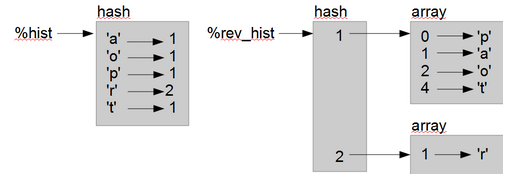
\includegraphics[scale=0.8]{figs/hash1.png}}
\caption{State diagram.}
\label{fig.hash1}
\end{figure}

Figure~\ref{fig.hash1} is a state diagram showing \verb'%hist'  and \verb'%rev-hist' .
A hash is represented as a box with the type {\tt hash} above it
and the key-value pairs inside.
\index{state diagram}
\index{diagram!state}

Arrays can be values in a hash, as this example shows, but they
cannot be keys.  If you try, you're likely to end up with a 
key that contains only one item of the array, but most likely 
not what you intended:

\begin{verbatim}
my @a = 'a' .. 'c';
my %h;
%h{@a} = 5;
say %h;  # -> a => 5, b => (Any), c => (Any)
\end{verbatim}

Here, Raku interpreted the \verb'%h{@a} = 5;' assignment 
as a a slice assignment, i.e., assumed that we were 
trying to populate three items in one go, one for each 
element of the array.

\index{hash!function}
\index{hashable}
As mentioned earlier, a hash is implemented using
a hashing function and that means that the keys have to 
be \emph{hashable} \footnote{This is not entirely true. The 
keys of a ``normal'' hash must be hashable and therefore 
immutable. There is another type of hash, object hashes, 
for which the need to have immutable keys does not apply.}. 
A {\bf hashing} is a function that takes 
a value (of any kind) and returns an integer.  Hashes use 
these integers, called hash values, to store and look up 
key-value pairs.
\index{immutability}

This system works fine if the keys are immutable.  But if the
keys are mutable, like with arrays, bad things would happen. For example,
when you create a key-value pair, Raku would hash the key and 
store it in the corresponding location.  If you modify the
key and then hash it again, it would go to a different location.
In that case, you might have two entries for the same key,
or you might not be able to find a key.  Either way, the
hash wouldn't work correctly.

That's why keys have to be hashable, and why mutable types like
arrays aren't. So Raku will do something else that can be 
useful (such as creating three distinct hash items in the 
example above), but will not hash the array itself.

Since hashes are mutable, they can't be used as keys,
but they {\em can} be used as values, so that you can 
have nested hashes.

\section{Memos}
\label{memoize}
\index{memoize}
\index{cache}
\index{memo}
\index{Fibonacci}

If you played with the {\tt fibonacci} subroutine from
Section~\ref{one.more.example}, you might have noticed that 
the bigger the argument you provide, the longer the 
subroutine takes to run. Furthermore, the run time 
increases extremely quickly.
\index{Fibonacci!function}
\index{function!Fibonacci}

To understand why, consider Figure~\ref{fig.fibonacci}, which shows
the {\bf call graph} for {\tt fibonacci} with {\tt n=4}.

\begin{figure}
\centerline
{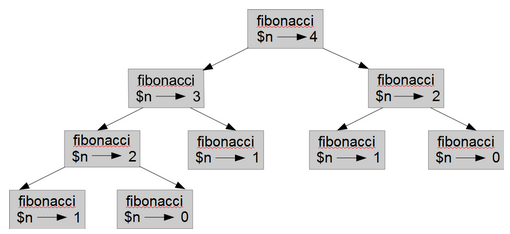
\includegraphics[scale=0.7]{figs/fibonacci.png}}
\caption{Call graph.}
\label{fig.fibonacci}
\end{figure}

A call graph shows a set of subroutine frames, with lines 
connecting each frame to the frames of the functions it 
calls.  At the top of the graph, {\tt fibonacci} with 
\verb'$n=4' calls {\tt fibonacci} with \verb'$n=3' and 
\verb'$n=2'.  In turn, {\tt fibonacci} with \verb'$n=3' calls
{\tt fibonacci} with \verb'$n=2' and \verb'$n=1'.  And so on.
\index{function frame}
\index{frame}
\index{call graph}

Count how many times {\tt fibonacci(0)} and {\tt fibonacci(1)} 
are called.  This is an inefficient solution to the problem, 
and it gets much worse as the argument gets bigger.
\index{memo}

One solution is to keep track of values that have already been
computed by storing them in a hash.  A previously computed value
that is stored for later use is called a {\bf memo}.  Here is a
``memoized'' version of {\tt fibonacci}:
\index{Fibonacci!memoized}

\begin{verbatim}
my %known = 0 => 1, 1 => 1;
say fibonacci(10);
sub fibonacci ($n) {
    return %known{$n} if %known{$n}:exists;
    %known{$n} = fibonacci($n-1) + fibonacci($n-2);
    return %known{$n};
}
\end{verbatim}
%

\verb'%known' is a hash that keeps track of the Fibonacci
numbers we already know.  It starts with
two items: 0 and 1, which both map to 1.

Whenever {\tt fibonacci} is called, it checks \verb'%known'.
If the result is already there, it can return
immediately.  Otherwise, it has to 
compute the new value, add it to the hash, and return it.

If you run this version of {\tt fibonacci} and compare it with
the original, you will find that it is much faster, especially 
for a large argument (say more than 30).

\index{cache}
\index{memoize}
Memoizing is a form of \emph{caching}, i.e., storing in memory 
the result of a (presumably costly) computing operation in 
order to avoid computing it again. This process is 
sometimes called ``trading memory against CPU cycles.''  In 
some cases, such as our Fibonacci recursive example here, the gain 
can be absolutely huge: calculating the 100th Fibonacci 
number would take billions of years with the original recursive 
subroutine and it takes only a split second with the memoized 
version.

Please note that in the specific case of the Fibonacci function, 
we are storing values for each successive integer; we could 
have memoized the Fibonacci numbers in an array rather than 
in a hash (and it might even be slightly more efficient), but 
using a hash for such purpose is a more general solution, 
working even when the memo keys are not consecutive integers.

As an exercise, try to rewrite the {\tt fibonacci} subroutine 
using an array instead of a hash to memoize the calculated 
Fibonacci numbers.


\section{Hashes as Dispatch Tables}
\label{dispatch}

You may 
need a procedure to launch some action depending on the 
value of a parameter received by the program. To do that, 
you could use a series of 
\verb'if {...} elsif {...} else {...}' 
statements like this:

\begin{verbatim}
sub run-stop  { ... };
sub run-start { ... };
my $param = get-param();
if $param eq "stop" {
    run-stop;
} elsif $param eq "start" {
    run-start;
} elsif $param = "h" {
    say $help;
} elsif $param = "help" {
    say $help;
} elsif $param = "v" {
    $verbose = True;
} else {
    die "Unknown option $param";
}
\end{verbatim}

This approach is boring and error-prone. Using a dispatch table 
is often a simpler solution.

A dispatch table is a data structure mapping identifiers to 
code references or subroutine objects. Applied to the 
above scenario, it could look like this:

\begin{verbatim}
sub run-stop  { ... };
sub run-start { ... };
my %dispatch = (
    stop  => &run-stop,
    start => &run-start,
    h     => { say $help; },
    help  => { say $help; },
    v     => { $verbose = True;},
);
my $param = get-param();
die "Unknown option $param" unless %dispatch{$param}:exists;
%dispatch{$param}(); # execute the action specified in %dispatch
\end{verbatim}

The \verb'%dispatch' hash defines the action depending on 
the parameter used as a key. The \verb'%dispatch{$param}()' 
statement calls the required action.

This approach is a bit more concise and slightly cleaner, but there 
are some other advantages. It is more maintainable: if you need 
to add one option, you just need to add one entry to the hash 
and don't have to add code in the middle of a complicated 
chain of nested \verb'if {...} elsif {...} else {...}' 
statements at the risk of breaking up something. 

Another upside is that the dispatch table can be dynamically 
modified at run time, for example depending on certain 
external circumstances (for example the day in the month when 
the program is running) or in accordance with a configuration 
file. This means that it is possible to dynamically modify 
the behavior of a program after compile time, while it is 
already running. This paves the way to some very interesting 
advanced programming techniques that are beyond the scope 
of this book.

Note that we have been using hashes for our dispatch tables, 
and this is the most common way to implement them. If it 
makes sense to have small integers as keys, you could also 
implement a dispatch table as an array. This is the case, 
for example, with numbered menu items where the user is 
prompted to type a number to indicate which menu option 
to activate.


\section{Global Variables}
\index{global variable}
\index{variable!global}
\index{lexical variable}
\index{variable!lexical}

In the memoized Fibonacci example above, the 
\verb'%known' hash is created outside the subroutine,
so it belongs to the whole main package.
Such variables are sometimes called {\bf global} 
because they can be accessed from any function.  Unlike ``local'' 
lexical variables, which usually disappear when their scope 
ends, global variables persist from one subroutine call to 
the next.
\index{flag}

It is common to use global variables for {\bf flags}; that is, 
boolean variables that indicate (``flag'') whether a condition
is true.  For example, some programs use a flag named 
\verb'$verbose' to control the level of detail in the
output:

\begin{verbatim}
my $verbose = True;
sub example1 {
    say 'Running example1' if $verbose;
    # ...
}
\end{verbatim}
%

Global variables are also sometimes used for environment 
variables and parameters passed to the program, as well
as for storing a large 
data structure that is the centerpiece of a program, in order 
to avoid copying it when passing it around as an argument to 
subroutines.

But, asides from those specific cases, it is usually 
considered poor practice to use a global variable, because 
it creates dependencies and unexpected ``action-at-a-distance'' 
behaviors between various parts of a program and may lead to 
difficult-to-track bugs.

In the case of our memoized \verb'fibonacci' subroutine, the 
\verb'%known' hash is useful only within the subroutine. We 
can improve the implementation by using the \verb'state' 
declarator within the subroutine:
\index{state}
\index{Fibonacci!memoized with a state variable}

\begin{verbatim}
say fibonacci(10);
sub fibonacci ($n) {
    state %known = 0 => 1, 1 => 1;
    return %known{$n} if %known{$n}:exists;
    %known{$n} = fibonacci($n-1) + fibonacci($n-2);
    return %known{$n};
}
\end{verbatim}
%
The \verb'state' declarator makes the variable local to the 
subroutine and persistent from one call to the subroutine to 
another: the code line with the \verb'state' statement is 
executed only once (at the first call of the subroutine) 
and the content of variable, the \verb'%known' hash in this 
case, is kept from one call to the next.



\section{Debugging}
\index{debugging}

As you work with bigger datasets it can become unwieldy to
debug by printing and checking the output by hand.  Here are some
suggestions for debugging large data sets:

\begin{description}

\item[Scale down the input] If possible, reduce the size of the
dataset.  For example if the program reads a text file, start with
just the first 10 lines, or with the smallest example you can find.
You can either edit the files themselves, or (better) modify the
program so it reads only the first {\tt n} lines.

If there is an error, you can reduce {\tt n} to the smallest
value that manifests the error, and then increase it gradually
as you find and correct errors.

\item[Check summaries and types] Instead of printing and checking the
entire dataset, consider printing summaries of the data: for example,
the number of items in a hash or the total of a list of numbers.

A common cause of runtime errors is a value that is not the right
type.  For debugging this kind of error, it is often enough to print
the type of a value (think about the {\tt .WHAT} method).
\index{WHAT}

It is often useful to add typing to your variables. Where you 
expect a string, make sure you type the variable or subroutine 
parameter with {\tt Str}. If you expect an integer, type it with 
{\tt Int}. If you expect an {\tt Int} of a certain range, create 
a subset for it as in Section~\ref{guardian} (p.~\pageref{guardian}) 
and type the variable with that.
\index{subset!type}
\index{type subset}

\item[Write self-checks:]  Sometimes you can write code to check
for errors automatically.  For example, if you are computing the
average of a list of numbers, you could check that the result is
not greater than the largest element in the list or less than
the smallest.  This is called a ``sanity check'' because it detects
results that are ``insane.''
\index{sanity check}
\index{consistency check}

Another kind of check compares the results of two different
computations to see if they are consistent.  This is called a
``consistency check.''

\item[Format the output] Formatting debugging output
can make it easier to spot an error.  We saw an example in
Section~\ref{factdebug}.  The {\tt dd} function displays 
helpful details on a composite or complex data structure.

\index{dd function}
\index{function!dd}

\end{description}

Again, time you spend building scaffolding can reduce
the time you spend debugging.
\index{scaffolding}


\section{Glossary}

\begin{description}

\item[Mapping] A relationship in which each element of one set
corresponds to an element of another set.
\index{mapping}

\item[Hash] A mapping from keys to their
corresponding values.
\index{hash}

\item[key-value pair:] The representation of the mapping from
a single key to its value.
\index{key-value pair}

\item[Item] In a hash, another name for a key-value
  pair.
\index{item!hash}

\item[Key] An object that appears in a hash as the
first part of a key-value pair.
\index{key}

\item[Value] An object that appears in a hash as the
second part of a key-value pair.  This is more specific than
our previous use of the word ``value.''
\index{value}

\item[Implementation] A way of performing a computation.
\index{implementation}

\item[Hash table] The algorithm used to implement hashes.
\index{hashtable}

\item[Hash function] A function used by a hash table to 
compute the location of a key.
\index{hash!function}

\item[Hashable] A type that has a hash function.  Immutable
types like numbers and strings are hashable; mutable types 
like arrays and hashes are not.
\index{hashable}

\item[Lookup] A hash operation that takes a key and finds
the corresponding value.
\index{lookup}

\item[Reverse lookup] A hash operation that takes a value and finds
one or more keys that map to it.
\index{reverse lookup}

\item[Call graph] A diagram that shows every frame created during
the execution of a program, with an arrow from each caller to
each callee. 
\index{call graph}
\index{diagram!call graph}

\item[Memo] A computed value stored to avoid unnecessary future 
computation.
\index{memo}

\item[Memoize] To store a computed value in memory to avoid having 
to recompute it. Memoizing is a form of caching.
\index{memoize}

\item[Global variable]  A variable defined outside any 
subroutine or other block.  Global variables can be 
accessed from any subroutine.
\index{global variable}

\item[Flag] A Boolean variable used to indicate whether a condition
is true.
\index{flag}

\end{description}


\section{Exercises}

\begin{exercise}
\label{wordlist2}
\index{set!membership}
\index{membership!set}

Write a subroutine that reads the words in \emph{words.txt} and
stores them as keys in a hash.  (It doesn't matter what the
values are.)  Then you can use the {\tt exists} adverb
as a fast way to check whether a string is in
the hash.

If you did Exercise~\ref{bisection}, you can compare the speed
of this implementation with a hash and the bisection search.

Solution: \ref{sol_wordlist2}

\end{exercise}


\begin{exercise}
\label{mem_ackerman}
Memoize the Ackermann function from Exercise~\ref{ackermann} 
and see if memoization makes it possible to evaluate the 
subroutine with bigger arguments.  Hint: no.
Solution: \ref{sol_mem_ackerman}.
\index{Ackermann function}
\index{function!ack}

\end{exercise}



\begin{exercise}
\index{duplicate}
\label{has_duplicates_hash}

If you did Exercise~\ref{has_duplicates}, you already have
a function named \verb"has-duplicates" that takes a list
as a parameter and returns {\tt True} if any object
appears more than once in the list.

Use a hash to write a faster, simpler version of
\verb"has-duplicates". 
Solution: \ref{sol_has_duplicates_hash}.

\end{exercise}


\begin{exercise}
\label{exrotatepairs}
\index{letter rotation}
\index{rotation, letters}

Two words are ``rotate pairs'' if you can rotate one of them
and get the other (see \verb"rotate_word" in 
Exercise~\ref{rotate}) using the Caesar cipher.
\index{Caesar cipher}

Write a program that reads a wordlist (e.g. {\tt words.txt} 
and finds all the rotate pairs.  
Solution: \ref{sol_exrotatepairs}.

\end{exercise}


\begin{exercise}
\label{homophones}
\index{Car Talk}
\index{Puzzler}

Here's another Puzzler from {\em Car Talk} 
(\url{http://www.cartalk.com/content/puzzlers}):

\begin{quote}
This was sent in by a fellow named Dan O'Leary. He came upon a common
one-syllable, five-letter word recently that has the following unique
property. When you remove the first letter, the remaining letters form
a homophone of the original word, that is a word that sounds exactly
the same. Replace the first letter, that is, put it back and remove
the second letter and the result is yet another homophone of the
original word. And the question is, what's the word?

Now I'm going to give you an example that doesn't work. Let's look at
the five-letter word, `wrack.' W-R-A-C-K, you know like to `wrack with
pain.' If I remove the first letter, I am left with a four-letter
word, 'R-A-C-K.' As in, `Holy cow, did you see the rack on that buck!
It must have been a nine-pointer!' It's a perfect homophone. If you
put the `w' back, and remove the `r,' instead, you're left with the
word, `wack,' which is a real word, it's just not a homophone of the
other two words.

But there is, however, at least one word that Dan and we know of,
which will yield two homophones if you remove either of the first two
letters to make two, new four-letter words. The question is, what's
the word?
\end{quote}
\index{homophone}
\index{reducible word}
\index{word, reducible}

You can use the hash from Exercise~\ref{wordlist2} above to check
whether a string is in {\tt words.txt}.

To check whether two words are homophones, you can use the CMU
Pronouncing Dictionary.  You can download it from
\url{http://www.speech.cs.cmu.edu/cgi-bin/cmudict}.
\index{CMU Pronouncing Dictionary}

Write a program that lists all the words in {\tt words.txt} 
(or in the CMU dictionary) that solve the Puzzler.
Solution: \ref{sol_homophones}.

\end{exercise}


